\newcommand\helampl{\mathcal{A}_{\vb*{\lambda}}}

In \cref{chap:stdtech,chap:numunitarity} we were operating on the objects under the assumption that they are Lorentz scalars.
However in QFT scattering amplitudes of particles with spin are not Lorentz scalars,
and the set of all Lorentz structures generated from Feynman diagrams is immensely redundant.
In this chapter we will discuss how amplitudes of any scattering process, 
polarized or not, can be decomposed into a minimal basis of Lorentz-invariant objects.

It is well known that the full physical information about any scattering process is contained in a complete set of \textit{helicity amplitudes} ---
the amplitudes with all external particles' states chosen to have a definite helicity (see the definition in \cref{chap:4dspinhel}).
Being non-redundant and complete representation of physical information, the helicity amplitudes 
enjoy a number of nice properties such as gauge invariance and manifestation of Poincaré symmetry.
On a technical side, the consequence is that the helicity amplitudes are expected to have the most compact representation,
given that they do not suffer from proliferation of unphysical information.
And indeed this has been shown to be the case in numerous practical applications (see e.g.\ %
\cite{DeLaurentis:2019phz,Badger:2019djh,Badger:2011yu,Badger:2013gxa,DeFreitas:2004kmi,Gehrmann:2011aa,Gehrmann:2009vu,Glover:2004si,Glover:2003cm,Garland:2002ak,Dunbar:2016aux,Dunbar:2016gjb,Dunbar:2016cxp,Badger:2015lda,Gehrmann:2015bfy,Bern:2003ck,Bern:2002tk,Badger:2018enw,Dunbar2017,Kunszt:1994nq}).

The computation of tree-level helicity amplitudes is a very straight-forward task,
which, from the perspective of Feynman diagrams,
amounts to simply inserting the corresponding states with definite helicities for each external particle.
The spinor-helicity techniques can be employed to further enhance the computations.
Moving forward to amplitudes with loops,
we are forced to make the dimensionality of space-time formally infinite \cite{Collins:1984xc} 
to regularize divergences.%
\footnote{
  A possibility to formulate the dimensional regularization in finite vector spaces was explored in \cite{Weinzierl:1999xb}.
  We do not pursue it here.
}%
\textsuperscript{,}%
\footnote{
  Other regularization methods are out of the scope of this thesis.
}
This fact makes both definition and evaluation of helicity amplitudes rather delicate.
It is the purpose of this chapter to present a concise and efficient method of
evaluating multi-loop helicity amplitudes in dimensional regularization,
amenable for numerical applications.

In \cref{sec:helampl_projectors} we briefly review a somewhat standard 
method of obtaining helicity amplitudes through $D$-dimensional projectors,
which can be found in the literature\footnote{
  see also related work in \cite{Chen:2019wyb,Boels:2018nrr} 
} \cite{Garland:2002ak, Moch:2002hm, Glover:2003cm, Glover:2004si,Gehrmann:2009vu,Gehrmann:2011aa}.
In \cref{sec:helampl_embeding}, 
taking advantage of some insights from \cref{chap:numunitarity},
we show how the tree-level approach of ``simply inserting appropriate external states'' can
be extended to loop amplitudes in the 't Hooft-Veltman (HV) flavor of dimensional regularization.
This allows to dispose of construction of complicated projectors, which
become vary hard to handle for large $(> 4)$ number of particles with spin \cite{Peraro:2019cjj}. 
Another convenient feature of our approach is that it can be applied in a numerical context, such
as evaluation of cuts through off-shell recursion as discussed in \cref{sec:evaluation_of_cuts}.
In \cref{sec:ds_reduction} we discuss how
the efficiency of extraction of the full $D_s$ dependence can be substantially improved
by dimensionally reducing kinematically-independent degrees of freedom in higher dimensions.

The content of this chapter is based on the parts of \cite{Anger:2018ove,Abreu:2018jgq,Abreu:2019odu}.

\section{Helicity Amplitudes}
\label{sec:HV_helicity_amplitudes}

A helicity amplitude $\helampl$
is defined as an $\mathcal{S}$-matrix element
with external polarization states $\varepsilon_{i}$ chosen to be
helicity eigenstates (for the definition of helicity see \cref{chap:4dspinhel}) with helicities $\vb*{\lambda}=\{\lambda_1,\ldots{},\lambda_N\}$.
Cross sections obtained from $\Abs{\helampl{}}$ describe
the scattering of polarized particles.
Unpolarized cross sections can be obtained by summing over the helicities of all external particles.
Helicity states satisfy the completeness relations
\begin{subequations}
  \label{eq:4d_completeness_relations}
  \begin{align}
    \sum_{\lambda=\{+1,-1\}} \varepsilon^\mu_\lambda(p){\varepsilon^\nu_\lambda}^{\star{}}(p)  &= -g^{\mu\nu} + \frac{p^\mu \eta^\nu + p^\nu \eta^\mu}{\sp(p,\eta)}, \\
    \sum_{\lambda=\{+\frac{1}{2},-\frac{1}{2}\}} u^\alpha_\lambda(p){\overline{u}_\lambda^\beta}(p)  &= \qty(\slashed{p}  \pm m\,\mathbb{1})^{\alpha\beta},
  \end{align}
\end{subequations}
for gauge bosons and fermions correspondingly.
The number of $N$-particle helicity amplitudes is thus $2^N$, but
the number of of independent analytic expressions can be further reduced by taking into account charge and parity transformations.

The transformation of helicity amplitudes under Lorentz boosts is completely specified by their 
external states, and is given by the \emph{little group scaling},
\begin{equation}
  \ket{p_i} \to t_i \ket{p_i}, \quad  \sket{p_i} \to \frac{1}{t_i} \ket{p_i} \implies \helampl \to  \qty(\prod_i t_i^{-2\lambda_i}) \helampl,
\end{equation}
where $t_i$ are complex phases.
As expected the squared matrix element $\Abs{\helampl{}}$ is Lorentz-invariant.
With the help of spinor helicity formalism we can also make any helicity amplitude itself into a scalar
by removing it's \emph{spinor weight} --- a factor which has the same little group scaling
as the helicity amplitude.
Hence the scalar objects we were operating on in \cref{chap:stdtech,chap:dshel} can be the normalized helicity amplitudes.

We can perturbatively expand helicity amplitudes in the coupling constants as
\begin{equation}
  \helampl =  \helampl^{(0)} + g^2 \helampl^{(1)} + g^4 \helampl^{(2)} + \ldots{},
\end{equation}
with all leading-order couplings absorbed into $\helampl^{(0)}$.
It is then convenient to use the tree helicity amplitude\footnote{if it is not vanishing} $\helampl ^{(0)}$ to remove the spinor weight
of loop amplitudes.
It should be noted that the definition of polarized cross sections may not depend on a regularization scheme
used to regularize divergences of loop amplitudes. This implies, that 
among the flavors of dimensional regularization only in the ones which consider external particles 
to be in four dimensions the helicity amplitudes can be consistently defined.

%This can be achieved for example by normalizing all amplitudes $A^{L}_N$ with $L\geq1$ by
%a corresponding tree amplitude $A^{0}_N$ 

\section{Form Factor Decomposition and Projectors}
\label{sec:helampl_projectors}

In this section we review the conceptually simplest way to define helicity amplitudes in dimensional regularization, which is through $D$-dimensional projectors.
This approach has been used in a number of computations (see e.g.\ \cite{Garland:2002ak, Moch:2002hm, Glover:2003cm, Glover:2004si,Gehrmann:2009vu,Gehrmann:2011aa}).
Its relation to HV scheme and helicity amplitudes has been recently discussed in \cite{Peraro:2019cjj}.

One starts with decomposing an amplitude with \emph{unspecified} external states into all possible $D$-dimensional tensor structures $\mathcal{T}_i$ compatible
with symmetries and gauge invariance,
\begin{equation}
  \mathcal{A}  = \sum_{i} \mathcal{T}_i\;A_i.
\end{equation}
For example $\mathcal{T}_i$ can contain object like $\sp(\varepsilon(p_i),p_j)$, $\bar{v}(p_i) \slashed{p}_j u(p_k) $, $\bar{u}(p_i) \slashed{\varepsilon}(p_j) u(p_k)$, etc.
Here $A_i$ are the Lorentz-invariant form factors.
Then one finds projectors $\mathcal{P}_i$ on $A_i$ from linear combinations of $\mathcal{T}_i$ by solving the equations
\begin{equation} \label{eq:cdr_projectors}
  \mathcal{P}_i [\mathcal{A}] = \qty(\sum_j c_{i,j}(\vb*{x},D) \sum_\text{(states)} \mathcal{T}^{\dagger}_j) \qty[\sum_{k} \mathcal{T}_k A_k] = A_i, 
\end{equation}
for the coefficients $c_{i,j}(\vb*{x},D)$, which are rational functions of external kinematics $\vb*{x}$ and $D$.
Here the state sums are taken to be in $D$ dimensions, which corresponds to working in the CDR scheme.

To extract the helicity amplitudes one then \textit{evaluates} the tensor structures $\mathcal{T}_i$ 
by inserting the corresponding \textit{helicity states in four dimensions} for each of the external particles. 
This is equivalent to switching to the HV scheme.
The procedure uncovers the fact that only particular linear combinations of $A_i$ are relevant,
and the number of these combinations is exactly the number of independent helicity amplitudes, which is
significantly lower than the number of initial tensor structures $\mathcal{T}_i$.

The difficulties of this approach are two-fold:
\begin{enumerate}
  \item The number of initial tensor structures grows very fast with the number of external particles with spin.
    This makes solving the equations \cref{eq:cdr_projectors} for projectors and then applying them to each Feynman diagram very challenging for $N>4$.
  \item The projectors have to be applied to analytic expressions since the external states in $D$ dimensions do not admit any finite numerical representations \cite{Collins:1984xc}.
\end{enumerate}

Since the helicity amplitudes contain the complete physical information, 
the construction of form factors in  \cref{eq:cdr_projectors} seems to be an unnecessary complication.
And indeed a way to avoid these steps and construct the projector onto helicity amplitudes directly has been suggested recently \cite{Peraro:2019cjj}.
This somewhat mitigates the first issue, but the projectors have to be still applied to analytic expressions.

\section{Helicity Amplitudes from Embedding of External States}
\label{sec:helampl_embeding}

In this section we explain how multi-loop helicity amplitudes
with vector and spinor external particles can be obtained in dimensional regularization
from appropriate embedding of helicity states into spaces of higher dimensionality $\mathsf{S}_{[D_s]}$.
As in \cref{sec:evaluation_of_cuts}, in this \namecref{chap:dshel} we will denote the dimensionality of particles'
representations as $D_s$.
Our approach is built up independently from the one described in the previous chapter, but we establish
the connection in the end.

In HV the space-time symmetry group is extended to $\mathrm{SO}(1,D_s-1)$, and the external particles are kept in four dimensions. 
More precisely this means that, like in CDR, the tensor and Clifford algebras are performed in $D_s$ dimensions,
but the completeness relations for external states have to be as in \cref{eq:4d_completeness_relations}. 
In other words the amplitudes in HV transform like their four-dimensional counterpart under $\mathrm{SO}(1,3)$, 
and are invariant under the rotations in $\mathrm{SO}(D_s-4)$. 
This implies that, upon normalizing by an appropriate spinor weight, the helicity amplitudes are scalars of the extended symmetry group $\mathrm{SO}(1,D_s-1)$.
In \cref{chap:numunitarity} we argued that we can use this symmetry to embed the formally infinite-dimensional computation
into a finite one with appropriately chosen integer values of $D^{(L)}$ and $D_s$.
This fact motivates our strategy:
\begin{enumerate}
  \item Consider amplitudes in arbitrary (integer) $D_s \geq  D^{(L)}$ dimensions with fixed external states,
    which have the right little-group behavior with respect to $\mathrm{SO}(1,3) \subset \mathrm{SO}(1,D_s-1)$.
  \item Impose the rotational symmetry in $\mathrm{SO}(D_s-4)$ by combining the degrees of freedom from $\mathsf{S}_{[D_s-4]}$ in
    a suitable way.
  \item Set $D_s\to D$ in the amplitudes obtained from the previous step (which are polynomials in $D_s$).
\end{enumerate}
As we will see shortly, the second step is trivial for vector particles. For fermionic
particles it requires a tensor decomposition similar to the one we discussed in \cref{sec:helampl_projectors},
but enormously simplified by the fact that the indices in  $\mathsf{S}_{[D_s-4]}$ are completely decoupled from kinematics\footnote{
  this applies after the loop integrations are performed, 
  but we can always pull the corresponding projectors into the integrand given that $D_s$ was not set to $D$ yet.
}
and that we can ignore all vector particles.



\subsection{Embedding of Vector States}
\label{sec:embedding_vectors}
Consider the amplitudes for the scattering of massless vector particles.
There are $(D_s - 2)$ states for each particle in $D_s$ dimensions. 
The corresponding polarization sum for a particle with momentum $p$ is 
\begin{equation} \label{eq:vector_pol_sum_ds}
  \sum_{j=1}^{D_s-2} \varepsilon^\mu_j(p){\varepsilon^\nu_j}^{\star{}}(p) = -g_{[4]}^{\mu\nu} + \frac{p^\mu \eta^\nu + p^\nu \eta^\mu}{\sp(p,\eta)} \;-\; g_{[D_s-4]}^{\mu\nu}, 
\end{equation}
where we used $p \in \mathsf{S}_{[4]}$
to make the $(D_s-4)$-dimensional part explicit.
Comparing this to \cref{eq:4d_completeness_relations} we see that we can embed the helicity states as \cite{Kosower:1990ax}
\begin{align} \label{eq:embedding_vectors}
  \varepsilon_{1,2}^\mu =
    \begin{dcases}
      \varepsilon^\mu_{+,-}, & \mu\in \mathsf{S}_{[4]},\\
      0, & \mu\in \mathsf{S}_{[D_s-4]},\\
    \end{dcases}
    &&
  \varepsilon_{j}^\mu = \delta^{(j+2)}_\mu, \qfor j\geq 3,
\end{align}
Thus the amplitudes in $D_s$ dimensions with $\varepsilon_{1,2}^\mu$ as external states satisfy the correct little-group scaling trivially.
If we now also take into account the orthogonality relations 
\begin{align}
  g_{[D_s]}^{\mu\nu} = g^{\mu\nu}_{[4]}+g^{\mu\nu}_{[D_s-4]}, && (g_{[4]})^{\mu\rho}(g_{[D_s-4]})_{\rho\nu} = 0,
      %& (g_{[x]})^{\mu}_\mu =x, \qfor x \in  \{4,D_s,D_s-4\},
\end{align}
we see that these amplitudes are invariants under the rotations in $\mathsf{S}_{[D_s-4]}$.
Hence they are the helicity amplitudes in the HV scheme.
This is, of course, a well-known fact which has been exploited in one-loop computations with numerical generalized
unitary methods \cite{Ellis:2007br,Giele:2008ve}, as well as as 
in the so-called six-dimensional helicity formalism \cite{Bern2011,Cheung:2009dc,Badger:2013gxa,Badger:2017jhb}.

Note that, in contrast to the form factor decomposition in \cref{sec:helampl_projectors}, we did not need any projectors.

\subsection{Embedding of Spinor States}
\label{sec:embedding_spinors}

We now consider amplitudes with external fermions.
There are $2^{\frac{D_s}{2}-1}$ spinor states in $D_s$ dimensions, 
which can be constructed through the representations of Clifford algebras (see \cref{sec:clifford_algebra_ds}).
The polarization sum with the momentum $p \in \mathsf{S}_{[4]}$ is
\begin{equation} \label{eq:ds_spin_polsum}
  \sum_{j=1}^{2^{\frac{D_s}{2}-1}} u^\alpha_j(p){\overline{u}_j^\beta}(p) = \qty(\slashed{p}_{[D_s]}  \pm m\,\mathbb{1}_{[D_s]})^{\alpha\beta} \equiv 
  \qty(\slashed{p}_{[4]} \pm m \cdot \mathbb{1}_{[4]})^{\bar{\alpha}\bar{\beta}} \qty(\mathbb{1}_{[D_s-4]})^{\hat{a}\hat{b}},
\end{equation}
where the indices $\alpha = \bar{\alpha}\otimes\hat{\alpha}$,  $\beta = \bar{\beta}\otimes \hat{\beta}$ are factorized into 
$\{\bar{\alpha},\bar{\beta}\}\in \mathsf{S}_{[4]}$ and $\{\hat{\alpha},\hat{\beta}\}\in \mathsf{S}_{[D_s-4]}$.
Comparing to \cref{eq:4d_completeness_relations}, we see that we can embed the four-dimensional spinors as
\begin{align} \label{eq:fermionicStates}
    \qty(u_{\lambda,i})^{\bar{\alpha}\hat{\alpha}} =  u_{\lambda}^{\bar{\alpha}} \cdot \delta_i^{\hat{\alpha}}, && i = 1,\ldots{},2^{\frac{D_s}{2}-2},
\end{align}
where we replaced the index $j$ in \cref{eq:ds_spin_polsum} by $\{\lambda, i \}$ to make the four-dimensional helicity $\lambda \in  \{+\frac{1}{2},-\frac{1}{2}\}$ manifest.
Thus the amplitudes in $D_s$ dimensions with any of the spinors $\qty(u_{\lambda,i})^{\bar{\alpha}\hat{\alpha}}$ taken as external fermionic states\footnote{
  The fact the these spinors also satisfy the Dirac equation in $D_s$ dimension can be easily verified.
}
(and with the vector states taken as in \cref{sec:embedding_vectors}) have the correct little-group scaling.
However, as opposed to the case of vector particles, we observe that 
all of the states in \cref{eq:fermionicStates} introduce a \emph{preferred direction} in  $\mathsf{S}_{[D_s-4]}$
via the indices $\hat{\alpha}$.
Hence the amplitudes with a particular choice of $\qty(u_{\lambda,i})^{\bar{\alpha}\hat{\alpha}}$ are \textbf{not} symmetric under the rotations $\mathrm{SO}(D_s-4)$.
From a different point of view, we have many states with the same helicity, which creates an ambiguity as to what 
should be the helicity amplitude.
On that account, we turn to the tensor decomposition of indices $\hat{\alpha}$.

\subsection{Tensor Decomposition in $D_s-4$}
\label{sec:HelAmplHV}

We decompose an amplitude with external fermions in $D_s$ dimensions as
\begin{equation} \label{eq:tensorDecomposition}
  \mathcal{A} = \sum_n v_n A_n,
\end{equation}
where all spinor indices $\hat{\alpha}_i \in \mathsf{S}_{[D_s-4]}$ (and only them) are absorbed into $v_n$,
and, consequently, $A_n$ are scalars of $\mathsf{S}_{[D_s-4]}$.
In the following we will show how to construct a convenient basis of the tensor structures $v_n$ 
for any number of external fermions.

First we observe that only the spinor chains of the form
\begin{equation} \label{eq:generic_dsm_4_schain}
  u^{\hat{\alpha}}_i \; \qty( \prod_k \gamma^{\mu_k}_{[D_s -4 ]} )^{\hat{\alpha}\hat{\beta}} \; u^{\hat{\beta}}_j \quad\equiv\quad 
  \qty( \prod_k \gamma^{\mu_k}_{[D_s -4 ]} )^{i j},
\end{equation}
with indices $\mu_i \in \mathsf{S}_{[D_s -4]}$ contracted to other spinor chains, contribute to $v_n$.
This is the consequence of the following facts:
\begin{itemize}
  \item Thanks to our choice of states for vector particles, all Lorentz vectors, which can be contracted with $\gamma^{\mu_i}_{[D_s]}$,
    project them into $\mathsf{S}_{[4]}$:
    \begin{align} \label{eq:trivialTens1}
      a_{\mu}
      \left( \gamma_{[D_s]}^\mu \right)_{\bar{\alpha}\hat{\alpha}}^{\bar{\beta}\hat{\beta}} =
      a_{\mu}\left(\gamma_{[4]}^\mu \right)_{\bar{\alpha}}^{\bar{\beta}} \delta_{\hat{\alpha}}^{\hat{\beta}}\,,
      &&
      a \in \{p_i,\varepsilon_{1,2}(p_i)\}
    \end{align}
    This has an effect that no kinematics-dependence can enter $v_n$.
  \item Any Lorentz indices inside the same spinor chain can be contracted yielding  
    \begin{equation} \label{eq:trivialTens2}
      \left(\gamma_{[D_s]}^\mu\right)_{\bar{\alpha}\hat{\alpha}}^{\bar{\kappa}\hat{\kappa}}
      \left(\gamma_{[D_s]\mu}^{\phantom{\mu}}\right)_{\bar{\kappa}\hat{\kappa}}^{\bar{\beta}\hat{\beta}}
      =D_s~\delta_{\bar{\alpha}}^{\bar{\beta}}\delta_{\hat{\alpha}}^{\hat{\beta}}\,.
    \end{equation} 
  \item Due to the factorized representation of the Clifford algebra (see \cref{eqn:cliffordrecursion}), any spinor chain can be written in a factorized form.
\end{itemize}
Non-trivial tensors $v_n$ are thus obtained by contracting
Lorentz indices between multiple chains of  matrices $\gamma_{[D_s-4]}$.
Some examples of possible $v_n$ are
\begin{equation}
  \begin{aligned}
    & \delta^{i_1}_{j_1} \delta^{i_2}_{j_2},\\
    & (\gamma_{[D_s-4]}^{\mu_1} )_{i_1}^{j_1} (\gamma_{[D_s-4]\mu_1}^{\phantom{\mu}})_{i_2}^{j_2}, \\
    & (\gamma_{\mu_1[D_s-4]}^{\phantom{\mu}} )_{i_1}^{j_1} (\gamma_{[D_s-4]}^{\mu_1}\gamma_{[D_s-4]}^{\mu_2} )_{i_2}^{j_2} (\gamma_{[D_s-4]\mu_2}^{\phantom{\mu}})_{i_3}^{j_3},\\
    & \qquad \vdots{}
  \end{aligned}
\end{equation}

To construct a basis of tensor structures $v_n$ we can decompose each of the spinor chains entering it
into the standard basis of anti-symmetrized products of gamma-matrices (see e.g.\ \cite{Veltman:1988au}),
\begin{align}\label{eq:basisGammaChainDs}
\gamma_{[D_s-4]}^{\mu_1 \ldots \mu_n} = \frac{1}{n!} \sum_{ \sigma\in S_n} \sgn(\sigma) \gamma_{[D_s-4]}^{\mu_{\sigma(1)}} \ldots \gamma_{[D_s-4]}^{\mu_{\sigma(n)}}\,,
\end{align}
where $S_n$ is the set of all permutations of $n$ integers, and $\sgn(\sigma)$ is the signature of the permutation $\sigma\in S_n$.
It can be shown (see \cref{sec:identities}), that the
projectors $\mathcal{P}_n$ onto $v_n$ can be constructed from the conjugated tensors $v_n^\dagger$ as
\begin{align} \label{eq:dsm_4_projectors}
  \mathcal{P}_n [v_m] \coloneqq \qty(\prod_{s=1}^{n_s} \Tr_s) v_n^\dagger\; v_m = c_n(D_s-4)~\delta_{n m},  %&& c_n = \frac{(D_s-4)!\,n!}{(D_s-4-n)!},
\end{align}
with the traces are taken over each of $n_s$ spinor chains, and we drop the irrelevant total factor of $\qty(\Tr\mathbb{1}_{[D_s -4 ]})^{n_s}$.
The coefficients $c_n$ can be computed for each $n_s$ combinatorially, as demonstrated in \cref{eq:cnCalc}.
We emphasize that, unlike the projectors in \cref{sec:helampl_projectors}, the ones in \cref{eq:dsm_4_projectors}
operate on the explicitly-represented objects, hence can be evaluated numerically.
We now consider two examples.

\paragraph{One pair of external fermions.}
As a first and trivial example we consider an amplitude with one pair of external fermions (and any number of external gauge bosons). 
There is only a single chain of matrices $\gamma_{[D_s-4]}$, so
there is only a single term in the decomposition of \cref{eq:tensorDecomposition},
\begin{equation}\label{eq:decompqqbar}
  \mathcal{A} =v_0\,A_0\,,\qquad \textrm{with}\quad (v_0)_{\hat{\alpha}}^{\hat{\beta}}=\delta_{\hat{\alpha}}^{\hat{\beta}}\,.
\end{equation}
\paragraph{Two pairs of distinct fermions.}
As a second example we consider an amplitude with two fermion pairs of different flavors, (and any number of gauge bosons). 
The basis $\{v_n\}$ consists of contractions between two spinor chains of the form \cref{eq:generic_dsm_4_schain}:
\begin{align}
  \begin{split} \label{eqn:4qtensors}
    (v_0)_{j_1j_2}^{i_1i_2}   = &
    \delta_{j_1}^{i_1} \delta_{j_2}^{i_2}\,, \\
    (v_1)_{j_1j_2}^{i_1i_2}=
    &(\gamma_{[D_s-4]}^{\mu_1} )_{j_1}^{i_1} 
    (\gamma_{[D_s-4]\mu_1}^{\phantom{\mu}})_{j_2}^{i_2}\,, \\
    & \vdots\\
    (v_k)_{j_1j_2}^{i_1i_2}=
    &(\gamma_{[D_s-4]}^{\mu_1 \ldots  \mu_k})_{j_1}^{i_1}
    (\gamma_{[D_s-4]\mu_1 \ldots \mu_k}^{\phantom{\mu}})_{j_2}^{i_2}\,,\\
    & \vdots\,
  \end{split}
\end{align}
The number of elements in the basis $\{v_n\}$ depends on $D_s$,
and is infinite for non-integer $D_s$ (because the basis of the Clifford algebra \cref{eq:basisGammaChainDs} is infinite).
But for any given number of loops $L$ only a finite number of basis elements $n^{(L)}\coloneqq \dim\{v_n\}$ can appear.
This number can be found from inspecting the diagrams without external gauge bosons 
with maximal number of propagators.
For instance we have $n^{(0)}=0$, $n^{(1)}=3$ and $n^{(2)}=5$.

Each coefficient $A_n$ in the decomposition of \cref{eq:tensorDecomposition} satisfies our desiderata 
of the HV amplitudes from \cref{sec:HV_helicity_amplitudes}, so, in principle, we need to determine all of them to obtain the full amplitude.
In the next section we argue that, at least to NNLO, it is not the case, 
and all physically-relevant information can be extracted from just one coefficient.  

\subsection{Relevant Coefficients}
\label{sec:relevant_tensors}

It was shown in \cite{Weinzierl:2011uz} that for NNLO computations only the $\order{\eps^0}$ terms of the 
\emph{finite remainders} $\mathcal{F}^{(1)}$ and $\mathcal{F}^{(2)}$ of one- and two-loop amplitudes are required.
They are defined by subtracting the universal divergent structure of one- and two-loop amplitudes, 
\begin{subequations}
  \begin{align}
    \label{eq:F0}
    \mathcal{F}^{(0)} &\coloneqq \mathcal{A}^{(0)}, \\ 
     \label{eq:F1}
    \mathcal{F}^{(1)} &\coloneqq \mathcal{A}^{(1)} - \mathbf{I}^{(1)} \mathcal{A}^{(0)}, \\ 
     \label{eq:F2}
    \mathcal{F}^{(2)} &\coloneqq \mathcal{A}^{(2)}  - \mathbf{I}^{(1)} \mathcal{A}^{(1)} - \mathbf{I}^{(2)} \mathcal{A}^{(0)}.
  \end{align}
\end{subequations}
The operators $\mathbf{I}^{(1)}$ and $\mathbf{I}^{(2)}$ can be found in \cite{Catani:1998bh,Sterman:2002qn,Becher:2009cu,Gardi:2009qi}.\footnote{
  We also include renormalization into these operators, which is possible in massless QCD.
  Alternatively we simply consider $\mathcal{A}^{(L)}$ to denote renormalized amplitudes in this section.
}
Here for convenience we also introduced a finite remainder for tree amplitudes, which is simply an alias for the amplitude itself.
We can expand both sides of \cref{eq:F0,eq:F1,eq:F2} in terms of tensor structures of \cref{eq:tensorDecomposition}
to get the corresponding coefficients $\mathcal{F}^{(i)}_n$ of the finite remainders.
The cross section is obtained by squaring the finite remainders, possibly multiplied by some
finite operator $\mathbf{F}$ (we refer to \cite{Weinzierl:2011uz} for details),
\begin{equation} \label{eq:Fsq}
  \Re\qty(\mathcal{F}^{\dagger(i)}\mathbf{F}\mathcal{F}^{(j)}) = \sum_m\sum_n\; \mathcal{P}_m \qty[v_n]  \; \Re\qty(\mathcal{F}^{\dagger(i)}_m\mathbf{F}\mathcal{F}^{(j)}_n) = 
     \sum_n c_n \; \Re\qty(\mathcal{F}^{\dagger(i)}_n\mathbf{F}\mathcal{F}^{(j)}_n),
\end{equation}
where in the last equality we used \cref{eq:dsm_4_projectors}.
For non-identical pairs of fermions\footnote{We discuss identical fermions below.} 
the first element of the basis $\{v_n\}$ is
\begin{equation}
  v_0  = \delta^{\hat{\alpha}_1}_{\hat{\beta}_1}\cdots \delta^{\hat{\alpha}_{n_s}}_{\hat{\beta}_{n_s}},
\end{equation}
and the corresponding coefficient $c_0 = 1$.
As demonstrated in \cref{sec:identities}, the coefficients of all other tensor structures
contribute to higher orders in $\eps$ when we set $D_s\to 4-2\eps$,
\begin{equation}
  c_i=\order{\eps}, \qfor i\geq 1,
\end{equation}
and we can drop all $\order{\eps}$ terms in \cref{eq:Fsq}.
Thus we conclude that all we need to know is the coefficient of $v_0$.


\subsubsection{Identical Fermions}
To illustrate how to handle the cases with identical fermions,
we consider an amplitude with two pairs of fermions with the same flavor. 
It can be constructed by anti-symmetrizing the corresponding amplitude with distinct flavors.
In this way, we start from the basis in \cref{eqn:4qtensors},
and extend it with anti-symmetrized tensors $\{\tilde v_n\}$ as
\begin{equation}\label{eq:basisIdentical}
	(\tilde v_n)_{j_1j_2}^{i_1i_2} \coloneqq  (v_n)_{j_1j_2}^{i_2i_1}\,,
\end{equation}
so our basis is now $\{v_n\}\cup \{\tilde{v}_n\}$.
It satisfies the following properties:
\begin{equation}\label{eq:dualBasisIdentical}
  \mathcal{P}_n[v_m]= c_n \delta_{m n}\,,\qquad
  \mathcal{\tilde{P}}_n[\tilde{v}_m]= \tilde{c}_n \delta_{m n}\,,\qquad
  \mathcal{P}_n[\tilde{v}_m] = \delta_{m 0}\,\delta_{n 0}+\mathcal{O}(\epsilon)\,.
\end{equation}
The coefficients in the first two equations are the same as for the case of distinct fermions. 
We do not provide the closed form for the coefficients in the last equation, but
we verified the fact that they are proportional to $(D_s-4)$ for $m,n>0$.

Now consider the interference between the two-loop finite remainder and 
the corresponding tree amplitude, which should be anti-symmetrized over flavors individually,
\begin{multline}
  \qty(\mathcal{F}^{(0)} - \mathsf{f}\circ\mathcal{F}^{(0)})^\dagger \cdot 
    \qty(\mathcal{F}^{(2)} - \mathsf{f}\circ\mathcal{F}^{(2)}) = \\
    \qty(\mathcal{P}_0\qty[\mathcal{F}^{(0)}] - \mathcal{P}_0\qty[\mathsf{f}\circ\mathcal{F}^{(0)}])^\dagger \cdot 
    \qty( \mathcal{P}_0\qty[\mathcal{F}^{(2)}] - \mathcal{P}_0\qty[\mathsf{f}\circ\mathcal{F}^{(2)}]) ~+~ \order{\epsilon}.
\end{multline}
Here the application of $f\circ$ exchanges the flavors. 
On the right hand side we used the identities from \cref{eq:dualBasisIdentical} to
show that, to $\order{\epsilon}$, 
we can anti-symmetrize the coefficients $\mathcal{F}_0$ of the remainders.
And the latter are computed as in the case of distinguishable fermions.

As another interesting application of these observations, we can explain why 
two different results for the two-loop helicity amplitudes of the four-quark scattering in QCD
from \cite{Glover:2004si} and \cite{DeFreitas:2004kmi} give the same
value for the finite remainder\footnote{The fact that the finite remainders agree was recognized by the authors of \cite{DeFreitas:2004kmi}.}.
The author of the former computed 
\[
  \mathcal{P}_0\qty[\mathcal{A}^{(2)}(q,\bar{q},Q,\bar{Q})],
\]
while the authors of the latter computed
\[
  \tilde{\mathcal{P}}_0\qty[\mathcal{A}^{(2)}(q,\bar{q},Q,\bar{Q})].
\]
Clearly these results will not be the same. 
However, taking into account the \cref{eq:dualBasisIdentical}, we get
\[
  \mathcal{P}_0\qty[\mathcal{F}^{(2)}] = \tilde{\mathcal{P}}_0\qty[\mathcal{F}^{(2)}] ~+~ \order{\epsilon}.
\]

\subsection{On Chiral Couplings}

It is well known, that dimensional regularization fails to regularize chiral theories consistently
(see e.g.\ \cite{Larin:1993tq,Boughezal:2019xpp,Jegerlehner:2000dz,Bonneau:1980yb,Bruque:2018bmy,Baikov:1991qz,Kreimer:1989ke}).
More colloquially this problem is known as ``the $\gamma_5$ problem'', because it is its analytic
continuation to $D$ dimensions which causes contradictions explicitly.
The dimensional regularization can still be employed in these models, 
but some additional manual interference is required in some cases. 

In this thesis we only consider two-loop amplitudes in pure QCD, so we do not have to explore the issue. 
Nevertheless we would like to comment on how our method of extraction of helicity amplitudes might be affected by it.
First of all, we emphasize that we \emph{did not} construct a new flavor of dimensional regularization,
and our results are that of the HV scheme.  So the discussion found in the literature applies to our results without modifications.
To this end, a prescription with  the ``four-dimensional'' $\gamma_5$ \cite{tHooft:1972tcz,Breitenlohner:1977hr,Larin:1993tq},
\[\commutator{\gamma_{5}}{\gamma^{\mu}_{[D_s]}}=0, \quad \forall \mu\geq 4,\]
can be trivially incorporated in our approach with the following:
\[
  \qty(\gamma_{5[D_s]})^{\bar{\alpha}\hat{\alpha}}_{\bar{\beta}\hat{\beta}} = \qty(\gamma^\star_{[4]})^{\bar{\alpha}}_{\bar{\beta}}\,\delta^{\hat{\alpha}}_{\hat{\beta}},
\]
and an explicit addition of counter-term contributions might be required.
Finally, it is worth mentioning that using the ``anti-commuting'' $\gamma_5$, that is
\[
  \anticommutator{\gamma_{5}}{\gamma^{\mu}_{[D_s]}}=0, \quad \forall \mu, \qquad\Longleftrightarrow\qquad \gamma_{5[D_s]} \equiv \gamma^\star_{[D_s]},
\]
in combination with dimensional reconstruction is not possible, since
in this case the amplitudes behave non-smoothly as functions of $D_s$ at all integer values due to the relation
\begin{equation}
  \Tr\qty(\gamma^\star_{[D_s]} \prod_{i=1}^{n} \gamma^{\mu_i}_{[D_s]}) \sim \delta^n_{D_s}.
\end{equation}


\subsection{Discussion}
\label{sec:dshel_discussion}

To summarize, the result of this section is the following algorithm for
a (numerical if desired) computation of helicity amplitudes in the HV scheme of dimensional regularization:
\begin{enumerate}[label={\arabic*.}]
  \item Evaluate amplitudes with all particles placed in generic $D_s \geq D^{(L)}$ dimensions (which can be finite integers for instance), 
    and the external gauge bosons and fermions embedded as given by \cref{eq:embedding_vectors,eq:fermionicStates}.
  \item Per each pair of external fermions take a trace over their indices $\{\hat{\alpha}_i,\hat{\beta}_i\} \in \mathsf{S}_{[D_s-4]}$ 
    to project onto the coefficient $\mathcal{A}_0^{(L)}$ of $\delta^{\hat{\alpha}_1}_{\hat{\beta}_1}\cdots \delta^{\hat{\alpha}_{n_s}}_{\hat{\beta}_{n_s}}$.
  \stepcounter{enumi}\item[(\arabic{enumi})]  If $D_s$ is set to a particular integer value (e.g.\ in a numerical computation),
    repeat with a sample of different $D_s$ values to reconstruct the polynomial dependence of $\mathcal{A}_0^{(L)}$ (see \cref{sec:dimensional_reconstruction}).
  \item Set $D_s\to D\to 4-2\eps$.
\end{enumerate}
This algorithm coincides with the one from \cite{Anger:2018ove}, where it was found from a different perspective.
It is rather straight-forward to see, that
helicity amplitudes obtained 
with our algorithm are exactly the same as the ones 
obtained following the prescription explained in \cref{sec:helampl_projectors}, 
as well as the result of the ``'t Hooft-Veltman algebra'' implemented in a \texttt{FORM} library ``Spinney'' \cite{Cullen2010}.
The difference is that our approach admits a direct numerical implementation, since it
operates on explicitly-represented finite objects.

We have implemented our algorithm in a \texttt{C++} framework for $D$-dimensional numerical unitarity computations 
of one- and two-loop helicity amplitudes to obtain the results presented in \cref{chap:wbb_pheno,chap:5parton}.
We also reproduced a number of results from the literature. 
The validity of the approach is thus thoroughly established by practical applications.

We conclude this section with some comments.
\paragraph{1.} 
The idea of embedding external states into higher-dimensional spaces to obtain
helicity amplitudes in dimensional regularization is not new. 
It has been employed in one-loop numerical unitary methods \cite{Ellis:2007br,Giele:2008ve}, as well as 
the six-dimensional helicity formalism \cite{Bern2011,Cheung:2009dc,Badger:2013gxa,Badger:2017jhb} for two loops.
However the embedding of fermionic states, in particular any number of them,
and the relation to the HV scheme were somewhat glossed over,
which caused some confusion in the past.

For example, instead of constructing invariants under the rotations in $\mathrm{SO}(D_s-4)$
with projections, one could attempt to simply consider a single embedding by
selecting $\hat{\alpha}_i=1$ in \cref{eq:fermionicStates} for all fermionic states.
In fact, for all one-loop amplitudes with any number of \emph{massless} external quarks,
this can be arranged \cite{Anger:2018ove}
to be equivalent to an explicit computation of traces.
In general, however, this will introduce a preferred direction in $\mathsf{S}_{[D_s-4]}$,
which breaks the rotational invariance, 
so the computation carried out this way does not correspond to the HV scheme.
This, in turn, implies that the components of loop momenta $\va{\mu}_i \coloneqq \ell^\mu_{i[D-4]}$ can explicitly appear in the integrands (see \cref{sec:ParamIntegrands} for some details),
and, strictly speaking, the argument we used for determining the minimal dimensionality $D^{(L)}$ for embedding of loop momenta is invalidated.
At one loop, this fact has been noticed in \cite{Fazio:2014xea,Badger:2017gta},
where it has also been proposed to remove these components from the integrands by hand.
The latter works for one-loop amplitudes with no more than one pair of \emph{massive} external quarks in addition
to any number of massless quarks.
In other cases $\order{\epsilon}$ differences with respect to amplitudes computed in HV will appear.
Starting from two loops the differences will appear already in poles in $\epsilon$. 

\paragraph{2.}
In this section we discussed the computation of loop amplitudes in the HV scheme, which addresses the divergences from loop integrals.
In the computation of observables (see \cref{eq:NNLO_xs}) also divergences from the integrals over unresolved phase space appear,
which are normally regulated by CDR.
In this regard, one might be worried that knowing the amplitudes in the HV scheme is not sufficient for phenomenological applications.
It turns out, that the amplitudes computed in the two different schemes can be converted into each other with the known transition rules \cite{Broggio:2015dga}.

\paragraph{3.}
In some places in our argument we referenced the little-group scaling 
of particles' states, which, strictly speaking, applies only when these states
are massless.
The helicity eigenstates can, of course, also be constructed for
massive particles as well, relative to some light-like reference spinor $\ket{q}$.
In this case the notion of the little-group scaling can be considered with respect
to this reference spinor \cite{Cohen:2010mi}.
Then all considerations in this chapter apply without any modifications.

 

\section{\texorpdfstring{$D_s$}{Ds} Dependence from Dimensional Reduction}
\label{sec:ds_reduction}

In this section we focus on the polynomial $D_s$ dependence of 
the coefficients $A^{(L)}_n$ in the tensor decomposition in \cref{eq:tensorDecomposition},
which we need to know analytically to be able to set $D_s=4-2\epsilon$ in the HV scheme.
In \cref{sec:dimensional_reconstruction} we explained the analytic dependence on $D_s$ 
can be reconstructed from numerical evaluations in several $D_s$ values.
Here we propose an alternative way of obtaining the coefficients of $D_s$ polynomials, 
inspired by dimensional reduction.
This represents an opportunity for a significant optimization, 
which is critical for amplitudes with external fermions.

The coefficients $A^{(L)}_n$ in \cref{eq:tensorDecomposition} are polynomials in $D_s$,
\begin{equation}
  A(D_s) = \sum_{i=0}^{N} \mathcal{K}_i~D_s^{i}\ .
  \label{eq:ds-poly}
\end{equation}
where $N$ is determined by the number of loops, tensor structure,
and a particular scattering process. 
In QCD we normally have $N=L - \#_f$ for $A^{(L)}_0$, 
where $\#_f$ is the number of closed fermion loops.

One way to obtain the coefficients $\mathcal{K}_i$ 
is with dimensional reconstruction (see \cref{sec:dimensional_reconstruction}).
This approach is conceptually straightforward and generic, 
but it has some drawbacks which we discuss in the following.
The dimensionality of vector representation of $\mathrm{SO}(1,D_s-1)$ scales linearly with $D_s$.
And the dimensionality of the representation of Clifford algebra scales exponentially as $2^{D_s/2}$.
Furthermore, in presence of fermions we can sample only even values for $D_s$,
which forces the values to be higher compared to the case of vector particles only.
For example, for two-loop QCD the minimal choice is $\{6,8,10\}$, and the number of components
of spinors is $32$ for $D_s=10$. 
This is a significant obstacle as far as numerical efficiency is concerned.
In addition we have to evaluate traces in \cref{eq:dsm_4_projectors} by explicit summation
over indices $\{\hat{\alpha}_i,\hat{\beta}_i\}$.
For amplitudes with $n_s$ pairs of external quarks this amounts to $(n_s \cdot 2^{\frac{D_s}{2}-2})$ contributions.
These issues can lead to a combined slowdown by a factor of $\sim 80$ 
for the evaluation of amplitudes with four quarks, relative to the amplitudes with only gluons.
Fortunately, this can be avoided with the technique that we discuss next.

First, we trivially rearrange \cref{eq:ds-poly} as
\begin{equation} \label{eq:ds-poly-alt}
  A(D_s) = \sum_{i=0}^{N} \tilde{\mathcal{K}}_i~\mathcal{D}^{i}, \qquad \mathcal{D} = D_s - D_0,
\end{equation}
where $D_0$ is some \textit{base} dimension, which we choose to be the smallest integer such that $ D_0 \geq D^{(L)} $ (e.g.\ $D_0=6$ for $L=2$ ).
Next we split the vector indices into direct sums, and spinor indices into direct products
with respect to $D_0$, exactly in the same way as we did with respect to $D_s=4$ in \cref{sec:helampl_embeding}.
For the metric tensor we get
\begin{align} \label{eq:ds-split-metric}
  g^{\mu\nu}_{[D_s]}  = g^{\mu\nu}_{[\mathcal{D}]} + g^{\mu\nu}_{[D_0]},  \qquad
  g^{\mu\nu}_{[\mathcal{D}]}g^{\phantom{\mu\nu}}_{\mu\nu\,[D_0]} = 0\,,
\end{align}
and for the gamma matrices,
\begin{equation} \label{eq:ds-gamma}
  (\gamma_{[D_s]}^\mu)_{a\kappa}^{\,b\lambda}  = \left\{ 
    \begin{array}{ll} 
      \left(\gamma_{[D_0]}^\mu\right)_a^{\;b} \,
      \delta_\kappa^\lambda\,, &\quad  0\le\mu \le D_0-1 \,,\\&\\
      \left(\gamma^\star_{[D_0]}\right)_a^{\;b} 
      \left(\gamma_{[\mathcal{D}]}^{(\mu-D_0)}\right)_\kappa^{\;\lambda}\,, 
      &\quad \mu \geq D_0 \,,
    \end{array}
    \right.
\end{equation}
Again, as in \cref{sec:helampl_embeding}, 
we can factorize all spinor chains, now with respect to $D_0$.
Then using the property
\[
  \Tr\qty(A \otimes B) = \Tr(A) \cdot \Tr(B),
\]
all traces required for the projections in \eqref{eq:dsm_4_projectors},
can be written as
\begin{equation} \label{eq:ds-split-traces}
  \Tr\left(\prod_{\mu_i\in \mathcal{G}}\gamma^{\mu_i}_{[D_s]}\right) =
  \Tr\left(\prod_{\mu_i\in \tilde{\mathcal{G}}}\gamma^{(\mu_i-D_0)}_{[\mathcal{D}]}\right) \cdot
  \Tr\left(\prod_{\mu_i\in \mathcal{G}}\gamma^{\mathfrak{I}(\mu_i)}_{[D_0]}\right).
\end{equation}
The product on the left hand side is over a sequence $\mathcal{G}$ of $D_s$-dimensional vector indices,
$\tilde{\mathcal{G}} = \{ \mu_i \in \mathcal{G} ~:~ \mu_i \geq D_0 \}$, and the map $\mathfrak{I}$ is defined as
\begin{equation}
  \mathfrak{I} : \mu \to
    \begin{cases}
      \mu, & 0\le\mu \le D_0-1\,, \\
      \star, & \mu \geq D_0\,.
    \end{cases}
\end{equation}
The traces in $\mathsf{S}_{[\mathcal{D}]}$ are evaluated with usual Clifford algebra to yield
\begin{equation} \label{eq:trace_d0}
  \Tr\qty(\prod_{i=1} \gamma_{[\mathcal{D}]}^{\tilde{\mu}_i}) =  \sum_\sigma \qty( c_\sigma \prod_{i,j} g_{[\mathcal{D}]}^{\tilde{\mu}_{\sigma_i}\tilde{\mu}_{\sigma_j}}),
\end{equation}
where the indices  $\tilde{\mu}_i$ are understood to be from $\mathsf{S}_{[\mathcal{D}]}$, and the sum is over all ways
of splitting the set of all indices $\{\tilde{\mu}_i\}$ into pairs.
Recall that $D_0\geq D^{(L)}$, which implies $\ell_i^\mu = 0$ for $\mu\geq D_0$.
The only other Lorentz vectors we have are external momenta and vector states, which only have non-vanishing components
in four dimensions. 
Therefore, metric tensors $g^{\mu\nu}_{[\mathcal{D}]}$ are the only objects with indices beyond $D_0$ we find
in the integrand after the evaluation of traces in  \cref{eq:trace_d0}.
Contracting these indices will produce terms of the form $g^\mu_{[\mathcal{D}]\mu} = \mathcal{D}$, 
and the expressions they are factors of will contribute to the coefficients $\tilde{\mathcal{K}}_i$ with $i>0$ in \cref{eq:ds-poly-alt}. 
The crucial observation is that in doing so we never touch external or loop kinematics.
This allows us to contract all these indices and distribute 
all diagrams contributing to the amplitude into coefficients $\tilde{\mathcal{K}}_i$ before
we do any other evaluations.
The remaining evaluations can then be performed in the base dimension $D_0$,
eliminating the problem of large representations.

\subsection{Diagrammatic Algorithm}
\label{sec:DsFeynRules}

In this section we illustrate how the decomposition \cref{eq:ds-poly-alt} can
be constructed systematically with an example of color-ordered QCD.

We apply the relations \labelcref{eq:ds-split-metric,eq:ds-gamma}
to the original Feynman rules  of the theory (see \cref{sec:cofr}) to obtain their dimensionally-reduced version
showed in \cref{tab:Ds-FeynRules}. 
Slightly abusing the terminology, we refer to the $\mathcal{D}$-dimensional gluon as the ``scalar'' 
both before and after the corresponding indices in $\mathsf{S}_{\mathcal{D}}$ are contracted.
\begin{table}[h]
  \centering
  \begin{minipage}[t]{0.4\textwidth}
  \begin{tabular}{cl}
    $\vcenter{\hbox{\hspace{-2ex}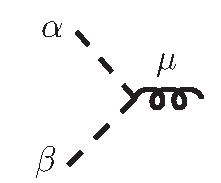
\includegraphics[width=13ex]{figures/Vssg}}}$ & $ \frac{i}{\sqrt{2}}(p_2-p_1)^\mu~ g^{\alpha\beta}_{[\mathcal{D}]}$ \\
    $\vcenter{\hbox{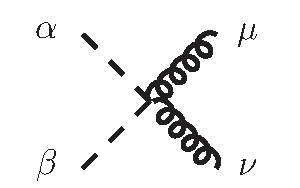
\includegraphics[width=15ex]{figures/Vssgg}}}$ & $ -\frac{i}{2}~g^{\mu\nu}_{[D_0]}~g^{\alpha\beta}_{[\mathcal{D}]}$ \\
    $\vcenter{\hbox{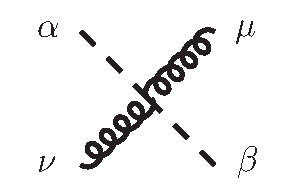
\includegraphics[width=15ex]{figures/Vsgsg}}}$ & $ i~g^{\mu\nu}_{[D_0]}~g^{\alpha\beta}_{[\mathcal{D}]}$ \\
  \end{tabular}
  \end{minipage}
  \quad
  \begin{minipage}[t]{0.5\textwidth}
  \begin{tabular}{cl}
    $\vcenter{\hbox{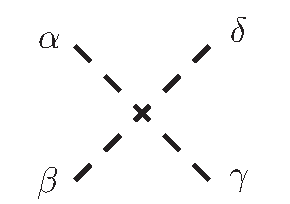
\includegraphics[width=15ex]{figures/Vssss1}}}$ &
      $
      \begin{aligned}
        i~g^{\alpha\gamma}_{[\mathcal{D}]} g^{\beta\delta}_{[\mathcal{D}]} - ~ & \\
                \frac{i}{2}~(g^{\alpha\beta}_{[\mathcal{D}]} g^{\gamma\delta}_{[\mathcal{D}]} & + g^{\alpha\delta}_{[\mathcal{D}]} g^{\beta\gamma}_{[\mathcal{D}]})
      \end{aligned}
      $ \\
        $\vcenter{\hbox{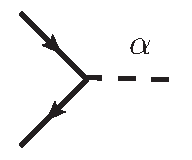
\includegraphics[width=11ex]{figures/VqqsR}}}$ & $- \frac{i}{\sqrt{2}}~\gamma^\star_{[D_0]} \gamma^\alpha_{[\mathcal{D}]}$ \\
        $\vcenter{\hbox{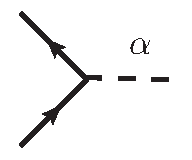
\includegraphics[width=11ex]{figures/VqqsL}}}$ & $ \frac{i}{\sqrt{2}}~\gamma^\star_{[D_0]} \gamma^\alpha_{[\mathcal{D}]}$ \\
  \end{tabular}
  \end{minipage}
  \caption{Color-ordered Feynman rules for vertices with scalars, which are introduced from dimensional reduction of gluons.}
  \label{tab:Ds-FeynRules}
\end{table}

To obtain the coefficients $\tilde{\mathcal{K}}_i$ in \cref{eq:ds-poly-alt} for an amplitude, we process each contributing  Feynman diagram with the following steps:
\begin{enumerate}
  \item Split all gluon lines in loops with \cref{eq:ds-split-metric} into a sum of $D_0$-dimensional gluon and a $\mathcal{D}$-dimensional gluon.
  \item Factorize all quark lines according to \cref{eq:ds-gamma}.
  \item Insert the Feynman rules from \cref{tab:Ds-FeynRules} and expand, keeping all $D_0$-dimensional objects untouched.
  \item Evaluate traces \eqref{eq:trace_d0}, and contract all $\mathcal{D}$-dimensional indices. 
     This replaces the $\mathcal{D}$-dimensional gluon by a scalar, and generates factors, which are polynomials in $\mathcal{D}$ with integer coefficients.
\end{enumerate}
An example of this procedure is given in \cref{fig:ds-example-diagram}.

\begin{figure}[ht]
  \newlength\diagramWidth
  \setlength{\diagramWidth}{18ex}
  \centering
  \begin{align*}
    \vcenter{\hbox{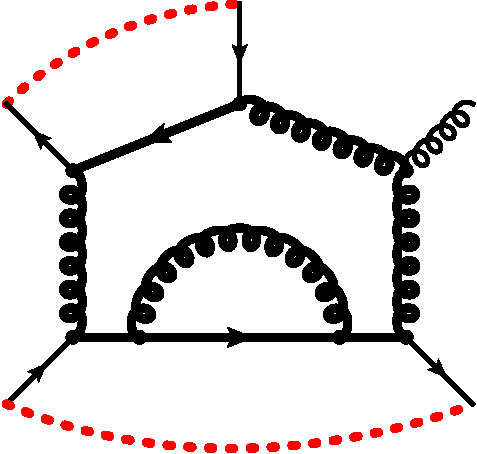
\includegraphics[width=\diagramWidth]{figures/Ds-example_B.pdf}}} \hspace{-10ex} & \hspace{15ex} = \hspace{6ex}
    \mathcal{D}^0 ~\cdot~ \vcenter{\hbox{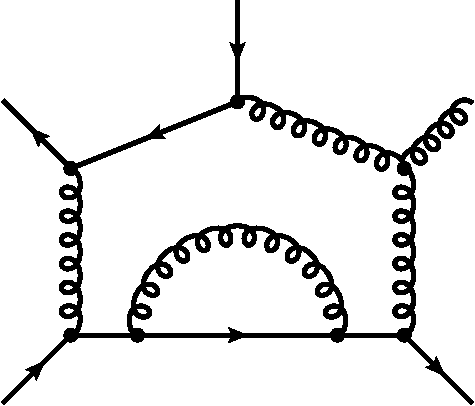
\includegraphics[width=\diagramWidth]{figures/Ds-example.pdf}}} \quad +\\
     & \mathcal{D}^1 ~\cdot~ \qty(~ 
    \vcenter{\hbox{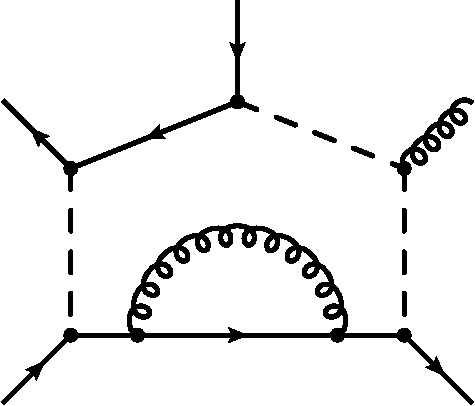
\includegraphics[width=\diagramWidth]{figures/Ds-example-1-1.pdf}}} \quad+\quad
    \vcenter{\hbox{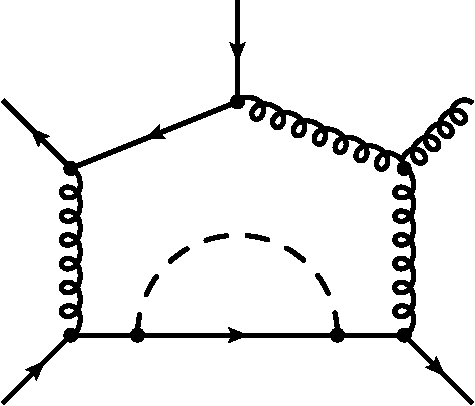
\includegraphics[width=\diagramWidth]{figures/Ds-example-1-2.pdf}}}
    ~) \quad +\\
     & \mathcal{D}^2 ~\cdot~ \quad \vcenter{\hbox{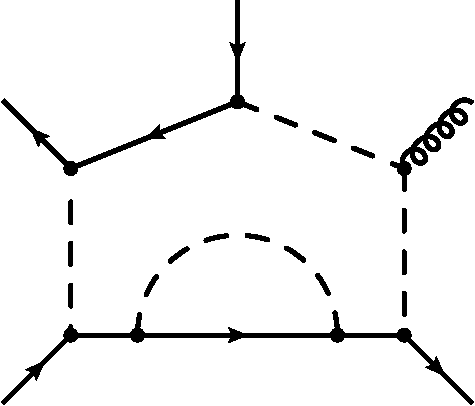
\includegraphics[width=\diagramWidth]{figures/Ds-example-2.pdf}}}
  \end{align*}
  \caption{Example of diagrams with scalar particles,
    representing the contributions to the coefficients of $\tilde{\mathcal{K}}_i$ in eq.~\eqref{eq:ds-poly-alt}.
    The thick lines in the diagram on the left-hand side represent particles in arbitrary $D_s$ dimensions.
    The (red) dashed represent the traces required for the projection in \cref{eq:dsm_4_projectors}.
    All particles on the right-hand side are $\mathcal{D}$-dimensional.}
  \label{fig:ds-example-diagram}
\end{figure}


Some comments are in order.
\begin{itemize}
  \item As a result of the algorithm presented above, all indices beyond $D_0$ are contracted.
    Taking the $\mathcal{D}$-dimensional traces, originated from the projections in \cref{eq:dsm_4_projectors}, was one of the prerequisites.
    These projections still need to be completed by evaluating the remaining traces over $(D_0-4)$-dimensional spinor indices,
    which can be done with explicit sums over the corresponding states, as in dimensional reconstruction.
  \item For two-loop amplitudes with no external fermions our method corresponds to the so called
six-dimensional helicity formalism \cite{Bern2011,Cheung:2009dc,Badger:2013gxa,Badger:2017jhb}.
From this point of view, our method can then be considered an extension thereof to amplitudes with fermions.
  \item Finally, although in this section we specialized to two-loop color-ordered QCD,
the generalization to different models and higher number of loops is straight-forward.
\end{itemize}



\subsection{Unitarity-Compatible Algorithm}
\label{dshel:sec:unitarity-compatible}

The algorithm for decomposition of amplitudes into $\mathcal{D}$ polynomials, 
described in the previous section, was formulated 
in terms of operating on individual Feynman diagrams.
In this regard, one might wonder if it can be employed together with
the numerical unitarity methods, where we evaluate
the products of tree amplitudes through the off-shell recursion, 
as discussed in \cref{sec:evaluation_of_tree_amplitudes}.
Here we explain how this can be done.

Instead of decomposing Feynman diagrams, 
we need to decompose \emph{cut diagrams}, 
i.e.\ the diagrams with vertices being tree amplitudes 
(see \cref{sec:evaluation_of_cuts} for details).
To this end, we process each cut diagram as follows:
\begin{enumerate}
  \item Perform the dimensional reduction of each vertex $V_{[D_s]i}$ of the cut diagram by applying steps 1 to 3 of the algorithm from the previous section,
    taking into account that only the gluons originating from the cuts contribute non-trivially.
    As a result, each vertex is expanded into a linear combination of the form
    \begin{equation}
      V_{[D_s]i} = \sum_k T_k^{\vb*{\alpha}} \; \tilde{V}_{[D_0]i}^{(k)},
    \end{equation}
    where $T_k^{\vb*{\alpha}}$ are the tensor structures of spinor and vector indices $\vb*{\alpha} \in \mathsf{S}_{[\mathcal{D}]}$.
    The new vertices $\tilde{V}_{[D_0]}^{(i)}$ ``remember'' 
    the tensor structures they originated from by allowing the dimensionally-reduced particles 
    to couple only in the way consistent with the corresponding tensor structure.\footnote{
      In the off-shell recursion this can be implemented by simply removing all currents which do not match the expected couplings.
    }
    Note that no restrictions are imposed on external gluons.
    We illustrate this step by an example shown in \cref{fig:example_dstree}.

    %, in addition to the list of external $D_0$-dimensional particles,
    %are identified by a restriction on how 
  \item Evaluate traces \eqref{eq:trace_d0}, and contract all $\mathcal{D}$-dimensional indices
    to bring the cut diagram to the form
    \begin{equation}
      \prod_i V_{[D_s]i} ~\to~  \sum_k c_k(\mathcal{D}) \prod_i \tilde{V}_{[D_0]i}^{(k_i)},
    \end{equation}
    which is then trivially rearranged into \cref{eq:ds-poly-alt}.  We give an example in \cref{fig:example_ds_cut2}.
\end{enumerate}

In this way the analytic $D_s$ dependence of each cut diagram is determined.
The reduction with numerical unitarity techniques of \cref{chap:numunitarity} 
can therefore be applied directly to the coefficients $\tilde{\mathcal{K}}_i$, which are evaluated in $\mathsf{S}_{[D_0]}$.

\begin{figure}[ht]
  \centering
  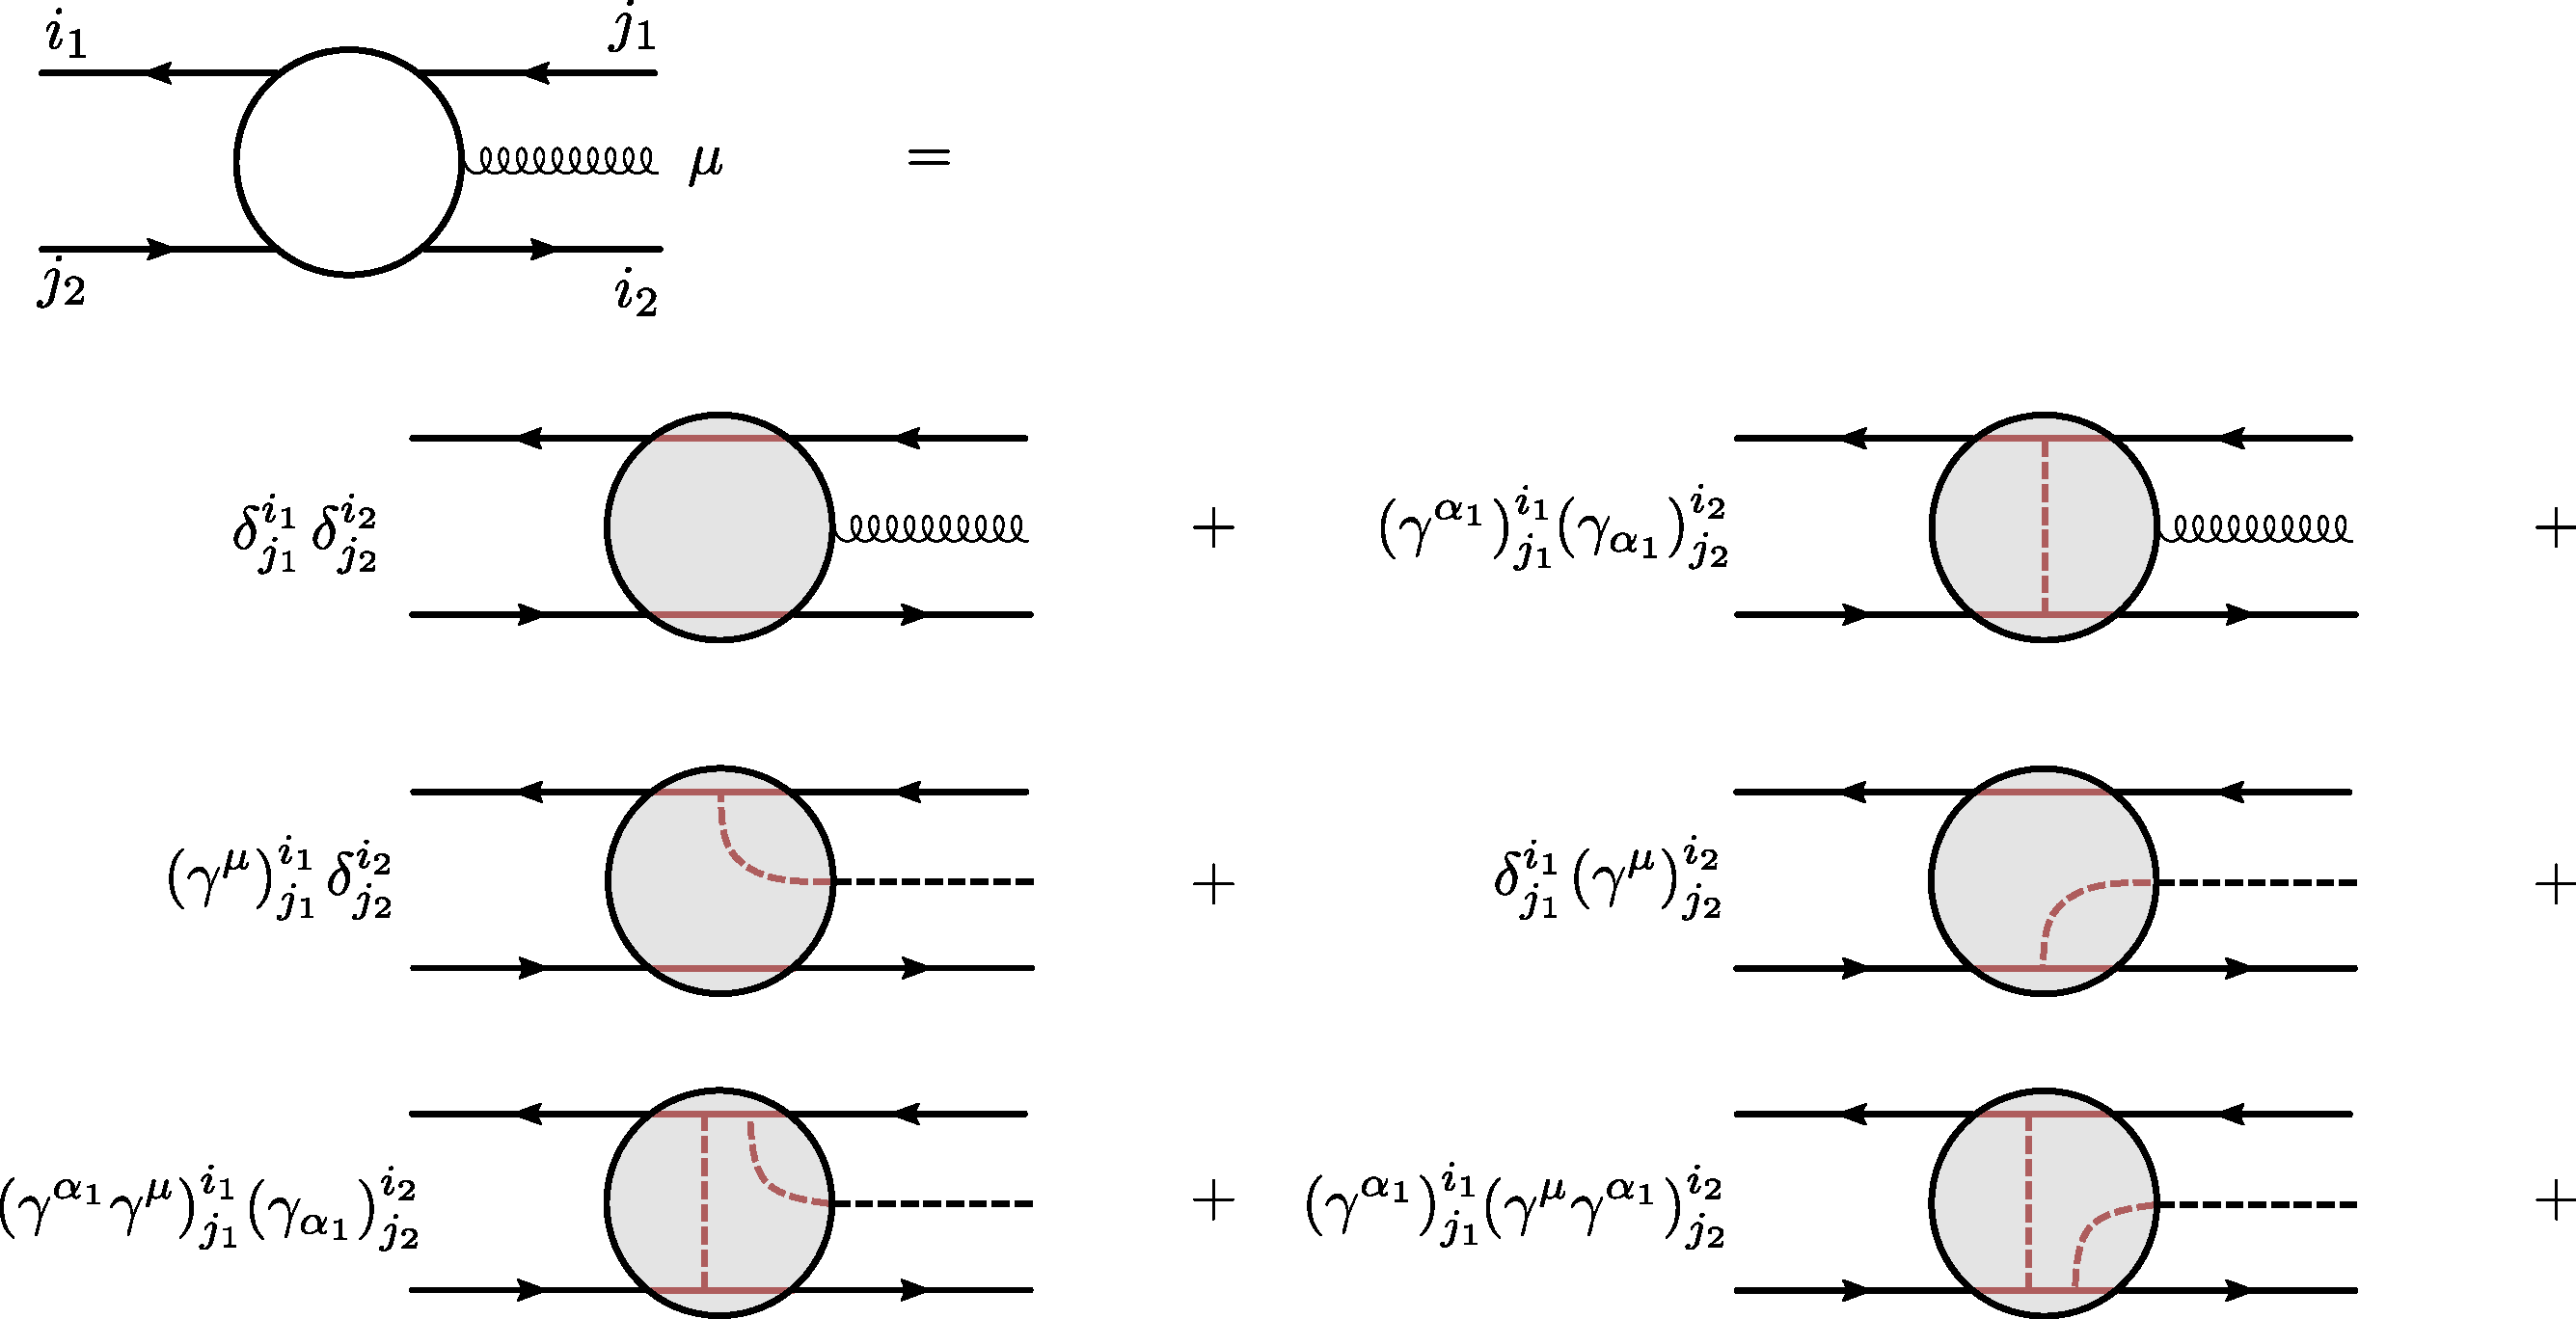
\includegraphics[width=0.9\textwidth]{example_dstree}
  \caption{An example of a dimensional reduction of a (color-ordered) 
    tree amplitude with particles in $D_s$ dimensions (on the left) into
    a linear combination of amplitudes in $D_0$ dimensions (on the right). 
    Only indices from $\mathsf{S}_{[\mathcal{D}]}$ are explicitly shown on the right.
    The shaded blobs specify subsets of diagrams with a particular coupling structure of the dimensionally-reduced particles, 
    which corresponds to the tensor structure in $\mathsf{S}_{[\mathcal{D}]}$.
  }
  \label{fig:example_dstree}
\end{figure}


\begin{figure}[ht]
  \centering
  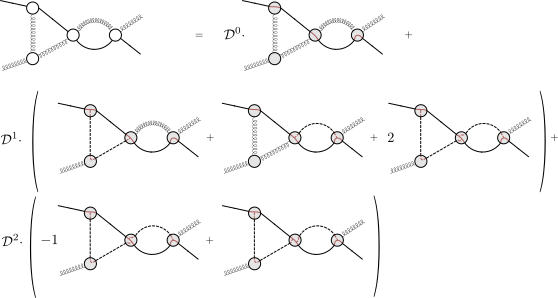
\includegraphics[width=1\textwidth]{example_ds_cut2}
  \caption{
    An example of the decomposition of a two-loop cut diagram in $D_s$ dimensions into coefficients $\tilde{\mathcal{K}}_i$ in \cref{eq:ds-poly-alt}.
    All diagrams on the right are in $D_0$ dimensions. The meaning of shaded blobs is as in \cref{fig:example_dstree}.
  }
  \label{fig:example_ds_cut2}
\end{figure}

